% =====================================================================
%  §5 Fukaya category and its degeneration  （原文 p28–p35，末句续至 p36 首）
% =====================================================================
\section{Fukaya 范畴及其退化}

\subsection{Fukaya 范畴}

在本文所采取的进路下，（紧辛流形的）Fukaya 范畴实际上将是一个 $\Ainf$-预范畴。我们的定义没有在最大的一般性下给出，但对于本文的主要应用——阿贝尔簇——已经足够。更精细的定义可参见 \cite{Fu1}、\cite{FuOOO}。

设 $(V,\omega)$ 是 $2n$ 维紧辛流形，且 $c_1(TV)=0\in H^2(V,\Z)$。与 $(V,\omega)$ 相伴的 Fukaya 范畴（取平凡 $B$ 场）还依赖于一些附加数据，下面我们逐一描述。

我们固定一个与 $\omega$ 相容的殆复结构 $J$，以及一个处处非零的光滑微分形式 $\Omega$，它关于 $J$ 是 $(n,0)$-形式。设 $L$ 是定向拉格朗日子流形。于是有映射
\[
  \mathrm{Arg}_L:=\mathrm{Arg}_{\Omega|_L}:L\longrightarrow \R/2\pi\Z,
\]
其中 $\mathrm{Arg}_{\Omega|_L}(x)$ 是非零复数 $\Omega(e_1\wedge\cdots\wedge e_n)$ 的辐角，而 $e_1,\dots,e_n$ 是 $T_xL$ 的一个定向基，$x\in L$。

\begin{dfn}
Fukaya 范畴 $\F(V,\omega,J,\Omega)$ 的对象是三元组 $(L,\rho,\widetilde{Arg}_L)$，其中 $L$ 是 $V$ 中带自旋结构的紧定向拉格朗日子流形（称为对象的支撑），$\rho$ 是 $L$ 上的局部系统（即带平坦联络的复向量丛），而 $\widetilde{Arg}_L:L\to\R$ 是 $\mathrm{Arg}_L$ 的连续提升。

我们要求：对任意元素 $\beta\in\pi_2^{\mathrm{free}}(V,L):=\pi_0(\mathrm{Maps}((D^2,\partial D^2),(V,L)))$，配对 $([\omega],\beta)$ 等于零。
\end{dfn}

我们有时把 Fukaya 范畴记作 $\F(V,\omega)$，或简记为 $\F(V)$。我们也常常省略提升后的辐角函数，从而把对象简记为 $(L,\rho)$。自旋结构的选取对于符号是本质的，而提升 $\widetilde{Arg}_L$ 的选取对于 $\Z$-分级是必要的。

\begin{yizhu}[Fukaya 范畴的对象]
这里把 Fukaya 范畴实现为 $\Ainf$-预范畴，是为了绕开 Floer 理论的一个技术困难：拉格朗日子流形之间未必横截，高阶复合只能在「横截序列」上定义，其延拓性质（命题 4）再由哈密顿形变来保证。三元组中的自旋结构用于给模空间以定向（从而确定符号），而 $\widetilde{Arg}_L$ 的提升用于 $\Z$-分级，二者都是 Floer 同调的经典技术输入。
\end{yizhu}

设 $\Ceps$ 由形式级数 $f=\sum_{i\ge0}c_ie^{-\lam_i/\eps}$ 组成，其中 $c_i\in\C$，$\lam_i\in\R$，$\lam_0<\lam_1<\cdots$，$\lam_i\to+\infty$。当 $[\omega]\in H^2(V,\Z)$ 时，实际上可以在域 $\C((q))$ 上工作，其中 $q=\exp(-1/\eps)$。一般地，我们给 $\Ceps$ 配备 adic 拓扑：零点的基本邻域系由集合
\[
  U_x=\Bigl\{f=\sum_{i\ge0}c_ie^{-\lam_i/\eps}\ \Bigm|\ \lam_i\ge x,\ i\ge 0\Bigr\},\qquad x\in\R,
\]
组成。

\begin{dfn}
对两个支撑横截的对象，我们如下定义态射空间
\[
  \begin{aligned}
  &\Hom_{\F(V,\omega)}\bigl((L_1,\rho_1,\widetilde{Arg}_1),(L_2,\rho_2,\widetilde{Arg}_2)\bigr)\\
  &\qquad:=\Bigl(\bigoplus_{x\in L_1\cap L_2}\Hom(\rho_{1x},\rho_{2x})\Bigr)\otimes\Ceps .
  \end{aligned}
\]
于是态射构成 $\Ceps$ 上的有限维向量空间。态射空间有一个 $\Z$-分级，它由 Maslov 指标 $\deg:L_1\cap L_2\to\Z$ 给出（见 \cite{Fu2}、\cite{Ko}、\cite{Se}）。Maslov 指标依赖于提升 $\widetilde{Arg}_L$ 的选取（它对应于拉格朗日 Grassmann 丛的万有覆盖中一个点的选取）。
\end{dfn}

\begin{rmk}
条件 $([\omega],\beta)=0$ 只是为了方便而引入的。它有助于避开我们前面提到的、关于复合 $m_0$ 的问题。当 $V$ 是带常值辛形式的环面、$L$ 是拉格朗日子环面时，该条件成立，而这是本文的主要应用。一般地，只要 $m_0$ 在 adic 拓扑下足够小，就有办法处理非平凡的 $m_0$。
\end{rmk}

下面我们描述 $\Ainf$-结构。它由一族分次向量空间的映射（高阶复合）
\[
  m_k^{F(V)}:\ \bigotimes_{0\le i\le k-1}\Hom_{\F(V)}\bigl((L_i,\rho_i),(L_{i+1},\rho_{i+1})\bigr)
  \ \longrightarrow\ \Hom_{\F(V)}\bigl((L_0,\rho_0),(L_k,\rho_k)\bigr)[2-k]
\]
给出，其中 $k\ge1$，而序列 $(L_0,\dots,L_k)$ 对应于一个横截的对象序列（后一概念将在下面定义）。

当所有局部系统都平凡且秩为一时，映射 $m_k$ 的定义如下。设 $D$ 是标准圆盘 $D=\{z\in\C\mid |z|\le1\}$。固定对象支撑的一个序列 $(L_0,\dots,L_k)$，使它们两两横截相交；再取交点 $x_i\in L_i\cap L_{i+1}$（$0\le i\le k-1$）与 $x_k\in L_0\cap L_k$，以及 $\beta\in\pi_2^{\mathrm{free}}(V,\cup_{0\le i\le k}L_i)$。我们用 $\MM(L_0,\dots,L_k;x_0,\dots,x_k;\beta)$ 记由下述组 $(y_0,\dots,y_k;\psi)$ 构成的集合：$y_i$（$0\le i\le k$）是 $\partial D$ 上按循环次序排列的互不相同的点，而 $\psi:D\to(V,J)$ 是伪全纯映射，满足
\[
  \begin{gathered}
  \psi(y_i)=x_i,\qquad \psi(\overline{y_iy_{i+1}})\subset L_i\quad (0\le i\le k),\\
  y_0=y_k,\qquad [\psi]=\beta .
  \end{gathered}
\]
这里 $\overline{y_iy_{i+1}}$ 表示 $y_i$ 与 $y_{i+1}$ 之间的弧。由分式线性变换在 $D$ 上的全纯作用，得到 $\mathrm{PSL}(2,\R)$ 在 $\MM(L_0,\dots,L_k;\allowbreak x_0,\dots,x_k;\beta)$ 上的自然作用。除 $k=1$、$x_0=x_1$、$\beta=0$ 这一对我们的目的无关的情形之外，该作用都是自由的。

\begin{yizhu}[局部系统与和乐因子]
与通常的 Fukaya 范畴不同，本文允许 $L$ 上任意（不必酉的）局部系统；这正是 \S1 提到的、在 Laurent 级数域上工作所带来的便利：和乐可以取任意值，而不必落在 $U(1)$ 中。$m_k$ 的每个求和项所乘的附加因子，就是局部系统沿圆盘边界各段弧的和乐之积。
\end{yizhu}

设 $x_i\in L_i\cap L_{i+1}$（$0\le i\le k-1$）、$x_k\in L_0\cap L_k$ 满足条件 $\deg x_k=\sum_{0\le i\le k-1}\deg x_i+2-k$。则矩阵元 $(m_k(x_0,x_1,\dots,x_{k-1}),x_k)$ 由公式
\[
  (m_k(x_0,x_1,\dots,x_{k-1}),x_k)=\sum\pm q^{(\beta,[\omega])}
\]
给出，其中求和遍历 $\MM(L_0,\dots,L_k;x_0,\dots,x_k;\beta)$ 中所有 $\mathrm{PSL}(2,\R)$-轨道。符号来自模空间 $\MM=\MM(L_0,\dots,L_k;x_0,\dots,x_k;\beta)/\mathrm{PSL}(2,\R)$ 中某些闭链的定向。我们将在下面加以评论（更多细节见 \cite{Fu1}、\cite{FuOOO}）。在局部系统非平凡的情形，每个求和项还多一个因子，它对应于局部系统沿各段弧的和乐。

下面描述横截性条件。设给定 Fukaya 范畴中对象的一个序列 $(L_i,\rho_i)$，$0\le i\le k$。若下列条件成立，我们就说它们是横截的：
\begin{enumerate}[label=\arabic*),leftmargin=2.2em,itemsep=2pt,topsep=3pt]
\item 只有两两之间的相交 $L_i\cap L_j$，且这些相交是横截的。
\item 对任意子序列 $(L_{i_0},\dots,L_{i_m})$（$m\ge1$，$i_0<i_1<\cdots<i_m$）与任意一组交点 $x_{i_m}\in L_{i_0}\cap L_{i_m}$、$x_{i_p}\in L_{i_p}\cap L_{i_{p+1}}$（$0\le p\le m-1$），只要
\[
  \deg x_{i_m}-\Bigl(\sum_{0\le p\le m-1}\deg x_{i_p}+2-m\Bigr)=0,
\]
则对任意 $\beta\in\pi_2^{\mathrm{free}}(V,\cup_{0\le p\le m}L_{i_p})$，模空间 $\MM(L_{i_0},\dots,L_{i_m};x_{i_0},\dots,x_{i_m};\beta)/\mathrm{PSL}(2,\R)$ 的相应分支只含光滑点，并且是零维的。
\item 若 $\deg x_{i_m}-\bigl(\sum_{0\le p\le m-1}\deg x_{i_p}+2-m\bigr)<0$，则相应分支为空。
\end{enumerate}

我们对这些条件略作说明（更多细节见 \cite{FuOOO}）。第一个条件是为了定义态射。第二个条件中出现的商集
\[
  \MM=\MM(L_{i_0},\dots,L_{i_m};x_{i_0},\dots,x_{i_m};\beta)/\mathrm{PSL}(2,\R)
\]
局部上可以等同于一个非线性椭圆问题的解空间。对于线性化问题，相应的 Fredholm 算子的指标为 $\deg x_{i_m}-\bigl(\sum_{0\le p\le m-1}\deg x_{i_p}+2-m\bigr)$。我们把 $\MM$ 的光滑点 $\MM^{sm}$ 定义为 Fredholm 算子余核平凡的那些点。于是 $\MM^{sm}$ 是维数等于该指标的光滑流形。此外可以验证，$\MM^{sm}$ 带有由相应 Fredholm 算子的行列式给出的自然定向，而正是在这里，$L_i$ 上自旋结构的选取进入了讨论。由此可知，在零维情形我们得到的是一个带重数 $\pm1$ 的点集（特别地，重数是整数）。在 Gromov--Witten 不变量的定义中出现、并产生非平凡分母的重覆盖与稳定映射，在本文的 Fukaya 范畴框架中并不出现（在我们的情形，虚拟次数为零的分支中所有「稳定映射」都是嵌入；分歧覆盖出现在更高的余维）。因此可以在环 $\Z_\eps$（$\Ceps$ 的整系数版本）上定义 Fukaya 范畴。带符号计点所得的数目给出 $m_k$ 的一个张量系数。

复合映射满足一组二次方程，从而使 $\F(V,\omega)$ 成为一个非幺 $\Ainf$-预范畴。可以验证，它事实上是一个 $\Ainf$-预范畴。延拓性质的证明基于 Fukaya 的如下结果（见 \cite{Fu2}、\cite{Se}）。

\begin{prp}
设 $(L_t,\rho_t)$ 是由 $\F(V)$ 的对象 $(L,\rho)$ 作小哈密顿形变得到的对象。则 $(L_t,\rho_t)$ 与 $(L,\rho)$ 是拟同构的。
\end{prp}

例如，由单个对象 $(L,\rho)$ 组成的序列可以延拓为横截序列 $\bigl((L_{t_1},\rho_{t_1}),(L,\rho)\bigr)$。类似地，任意有限个横截序列都可以延拓。

容易看出，对 $(J,\Omega)$ 构成的空间（赋以自然拓扑）而言，其连通分支之集是格 $H^1(V,\Z)$ 上的主齐性空间。具体地说，$f:V\to U(1)$ 如下作用在 $(J,\Omega)$ 上：$(J,\Omega)\mapsto(J,f\Omega)$。下面的定理可由 \cite{Fu2} 推出。

\begin{thm}
存在与 $\omega$ 相容的殆复结构空间中的一个第二纲集（Baire 意义下）$\Sigma$，使得只要 $J_1,J_2\in\Sigma$ 且 $(J_1,\Omega_1)$ 与 $(J_2,\Omega_2)$ 同伦，Fukaya 范畴 $\F(V,\omega,J_1,\Omega_1)$ 与 $\F(V,\omega,J_2,\Omega_2)$ 就等价。
\end{thm}

因此，Fukaya 范畴的等价类只依赖于这对数据所在空间的连通分支。

\begin{yizhu}[第二纲集]
第二纲集（set of the second category）是指不能表为可数个无处稠密集之并的集合。与 $\omega$ 相容的殆复结构构成的空间是一个 Baire 空间，其中的第二纲集即「一般位置」的集合，因此定理 1 应读作：对一般的 $J$，$\F(V,\omega,J,\Omega)$ 的等价类在相差同伦的意义下与 $J$、$\Omega$ 的具体选取无关。
\end{yizhu}

\begin{rmk}
本节的各项定义（以及本文其他各节的定义）都可以修改，以适应非零 $B$ 场的情形。为避免记号更加复杂，我们不这样做。
\end{rmk}

\subsection{环面纤维化的 Fukaya--Oh 范畴}

设 $(Y,g_Y,\nabla)$ 是带整仿射结构的 AK 流形。协变格仍如前面那样记作 $\TYZ$。今后我们假设 $Y$ 是紧的。这是一个很强的限制。\cite{CY} 证明了：在此情形，空间 $Y$ 的某个有限覆盖是带标准仿射结构的环面。这种情形出现在复阿贝尔簇的坍缩中。

\begin{yizhu}[AK 流形]
AK 流形即仿射凯勒流形（affine and K\"ahler manifold）：它是 \S3.2 中定义 2 的 Monge--Amp\`ere 流形去掉 Monge--Amp\`ere 方程这一条件后所得的对象（另见 \cite{CY}），带有平坦联络 $\nabla$、黎曼度量 $g_Y$ 与协变格 $\TYZ$。\S3 已说明，环面纤维化的对偶构造对 AK 流形同样适用。
\end{yizhu}

流形 $X^\vee=\Tstar_Y/(\TYZ)^\vee$ 是环面丛 $p^\vee:X^\vee\to Y$ 的全空间。它带有由 $\Tstar Y$ 上的标准辛形式诱导的自然辛形式 $\omega=\omega_{X^\vee}$。我们给 $X^\vee$ 配备与 $\omega$ 相容的单参数复结构族 $J_\eta$（$\eta\to0$）。事实上，流形 $X^\vee_\eta:=\Tstar_Y/\eta(\TYZ)^\vee$ 带有前面描述过的典范复结构。我们用映射 $(y,v)\mapsto(y,\eta v)$ 把 $X^\vee$ 与 $X^\vee_\eta$ 等同起来，其中 $y\in Y$、$v\in\Tstar_{Y,y}$。借助这个等同，把复结构与度量拉回到 $X^\vee$。对 $\eta$ 的所有取值，$p^\vee:X^\vee\to Y$ 的纤维都是平坦拉格朗日环面。

我们如下在 $(X^\vee,J_\eta)$ 上定义一个处处非零的 $(n,0)$-形式 $\Omega_\eta$。固定 $\Tstar_{Y,y}$（$y\in Y$）中的一个定向正交基 $e_1,\dots,e_n$。$\Omega_\eta$ 定义为 $X^\vee$ 上的 $n$-形式，它关于 $T^{\Z}_{Y,y}/(T^{\Z}_{Y,y})^\vee$ 的作用不变。它在每一点处的值由下式给出：
\[
  \bigwedge_{1\le j\le n}\bigl((p^\vee)^*e_j+\sqrt{-1}\,J_\eta(p^\vee)^*e_j\bigr).
\]

设 $L$ 是 $X^\vee$ 中的紧定向拉格朗日子流形，使 $p^\vee|_L$ 是非分歧覆盖，且 $L$ 的定向由 $Y$ 的定向诱导。我们断言，函数 $\widetilde{Arg}_L:L\to\R$ 有一个典范的选取 $\widetilde{Arg}_L^{can}:L\to\R$。事实上，对任意点 $x\in X^\vee$，$T_{X^\vee,x}$ 中与垂直切空间 $T^{vert}_x=\operatorname{Ker}(p^\vee)_*$ 横截的拉格朗日子空间构成的空间是可缩的。考虑由二元组 $(x,l)$ 构成的空间 $\LL$，其中 $x\in X^\vee$，而 $l\subset T_{X^\vee,x}$ 是与 $T^{vert}_x$ 横截、并带有由 $Y$ 诱导的定向的拉格朗日子空间。则函数 $(x,l)\mapsto\mathrm{Arg}_{(\Omega_\eta)|_l}(x)\in\R/2\pi\Z$ 有唯一的连续提升 $\widetilde{Arg}:\LL\to\R$，它在 $(x,J_\eta(T^{vert}_x))$（$x\in X^\vee$）处取零。把这个函数限制到 $L$，便得到 $\widetilde{Arg}_L^{can}$。

我们把 $\F(X^\vee,\omega,J_\eta,\Omega_\eta)$ 记作 $\F^\eta(X^\vee)$，并把它的满 $\Ainf$-预子范畴记作 $\F^\eta_{unram}(X^\vee)$，其对象为 $(L,\rho,\widetilde{Arg}_L^{can})$，其中 $L$ 是紧拉格朗日子流形，其定向由 $Y$ 诱导，$p^\vee|_L$ 是非分歧覆盖，而 $\widetilde{Arg}_L^{can}$ 如上所述。为简化记号，我们把这些范畴的对象记作 $(L,\rho)$。

\begin{rmk}
可以验证：对如上所述的两个横截拉格朗日子流形 $L_1$ 与 $L_2$，任意 $x\in L_1\cap L_2$ 处的 Maslov 指标等于光滑 Morse 函数 $f_1-f_2:Y\to\R$ 在 $p^\vee(x)$ 处的 Morse 指标，这里 $f_i$ 使得在 $x$ 的局部有 $L_i=\operatorname{graph}(df_i)\ \bigl(\mathrm{mod}\,(\TYZ)^\vee\bigr)$，$i=1,2$。
\end{rmk}

由 \cite{FuO} 的结果可知，$\Ainf$-预范畴族 $\F^\eta_{unram}(X^\vee)$（$\eta\to0$）在如下意义下有极限：$\F^\eta_{unram}(X^\vee)$ 的对象与态射不依赖于 $\eta$，在极限中保持不变；复合 $m_k^{\F^\eta_{unram}(X^\vee)}$ 当 $\eta\to0$ 时在 $\Ceps$ 的 adic 拓扑下有极限。这些极限将在下面显式描述。

下面的结果可由 \cite{FuO} 推出。

\begin{prp}
对充分小的 $\eta$，极限 $\Ainf$-预范畴与 $\F^\eta_{unram}(X^\vee)$ 等价。
\end{prp}

我们把这个 $\Ainf$-预范畴记作 $FO(X^\vee)$，并称之为 $X^\vee$ 的 Fukaya--Oh 范畴（或 $X^\vee$ 的退化 Fukaya 范畴）。

\begin{rmk}
以下我们假设 $\dim Y>1$。$\dim Y=1$ 的情形略有不同，但也简单得多（例如见 \cite{P1}）。特别地，在此情形 $\F^\eta_{unram}(X^\vee)$ 不依赖于 $\eta$。
\end{rmk}

如前面所说，$FO(X^\vee)$ 的对象与态射和 $\F^\eta_{unram}(X^\vee)$ 的相同。为定义复合映射
\[
  m_k:\bigotimes_{0\le i\le k-1}\Hom\bigl((L_i,\rho_i),(L_{i+1},\rho_{i+1})\bigr)
  \longrightarrow\Hom\bigl((L_0,\rho_0),(L_k,\rho_k)\bigr)[2-k],
\]
这里使用的仍是标准公式，只是求和遍历下面所描述的一类 $X^\vee$ 中的二维曲面。对 $FO(X^\vee)$ 中对象的一个序列 $\bigl((L_0,\rho_0),\dots,(L_k,\rho_k)\bigr)$（$k\ge1$），我们考虑浸入的二维曲面 $S\to X^\vee$，满足：
\begin{enumerate}[label=\alph*),leftmargin=2.2em,itemsep=2pt,topsep=3pt]
\item $S$ 的边界落在 $L_0\cup\cdots\cup L_k$ 中。
\item $S=(\cup_\alpha T_\alpha)\cup(\cup_\beta S_\beta)$，其中 $T_\alpha$ 是 $p^\vee$ 的纤维中的测地三角形，因而投影为 $Y$ 中的点。
\item 每个 $S_\beta$ 是含于 $p^\vee$ 的纤维中的一族单参数测地区间之并（即一条「条带」）。此外，$p^\vee|_{S_\beta}:S_\beta\to Y$ 是到 $Y$ 中浸入的连通区间 $I_\beta:=p^\vee(S_\beta)$ 上的纤维化。$S_\beta$ 在 $I_\beta$ 的内点上的纤维是长度严格正的测地区间；$S_\beta$ 在 $I_\beta$ 的边界点上的纤维，要么是三角形 $T_\alpha$ 的边，要么是交点 $x_i\in L_i\cap L_{i+1}$（$0\le i\le k-1$）、$x_k\in L_0\cap L_k$。
\item 区间 $I_\beta$ 是 $Y$ 中浸入的平面三价树 $\Gamma$ 的边。点 $p^\vee(T_\alpha)$ 是 $\Gamma$ 的内顶点，而 $\Gamma$ 的尾顶点是交点 $x_0,\dots,x_k$ 的投影。
\item 设 $r:\Tstar_Y\to X^\vee$ 是自然的沿纤维万有覆盖。若拉格朗日流形 $r^{-1}(L_i)$（$i=0,\dots,k$）局部上由 $Y$ 上光滑函数 $f_i$（$i=0,\dots,k$）的微分给出，则 $\Gamma$ 的边必须是 $f_i-f_j$ 的梯度流线。$r^{-1}(L_i)$ 与 $r^{-1}(L_j)$ 的交点对应于 $f_i-f_j$ 的临界点。
\end{enumerate}

下图画出一个典型的曲面：

\begin{center}
  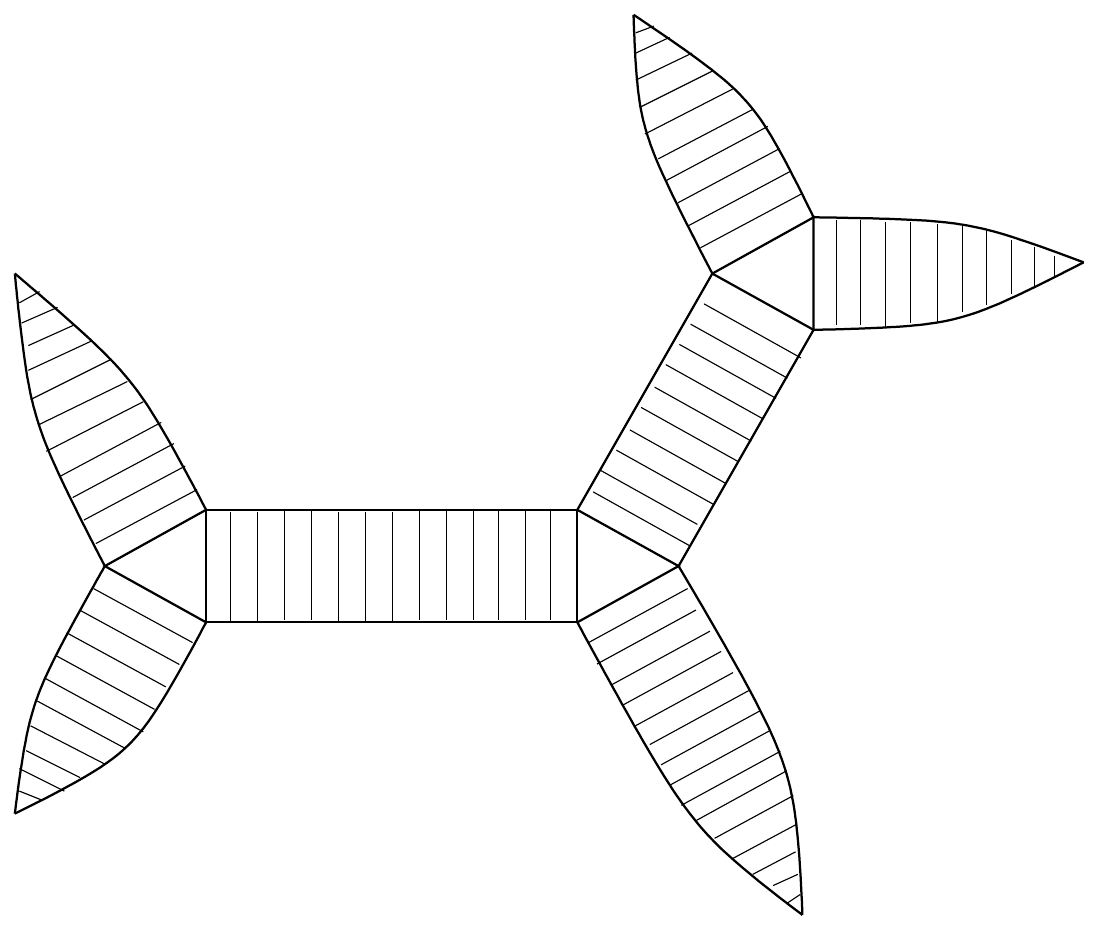
\includegraphics[width=4.64 cm]{figures/fig4_p34_surface_S}
\end{center}

曲面 $S$ 到 $Y$ 的投影是一棵梯度树，其尾顶点是 $f_i-f_{i+1}$ 或 $f_0-f_k$ 的临界点，边 $p^\vee(S_\beta)$ 是函数 $f_i-f_j$ 的梯度流线，其中 $i=i(\beta)$、$j=j(\beta)$、$i<j$。三角形被映到树的内顶点。对如上曲面 $S$，$\Gamma=p^\vee(S)$ 的图形如下：

\begin{center}
  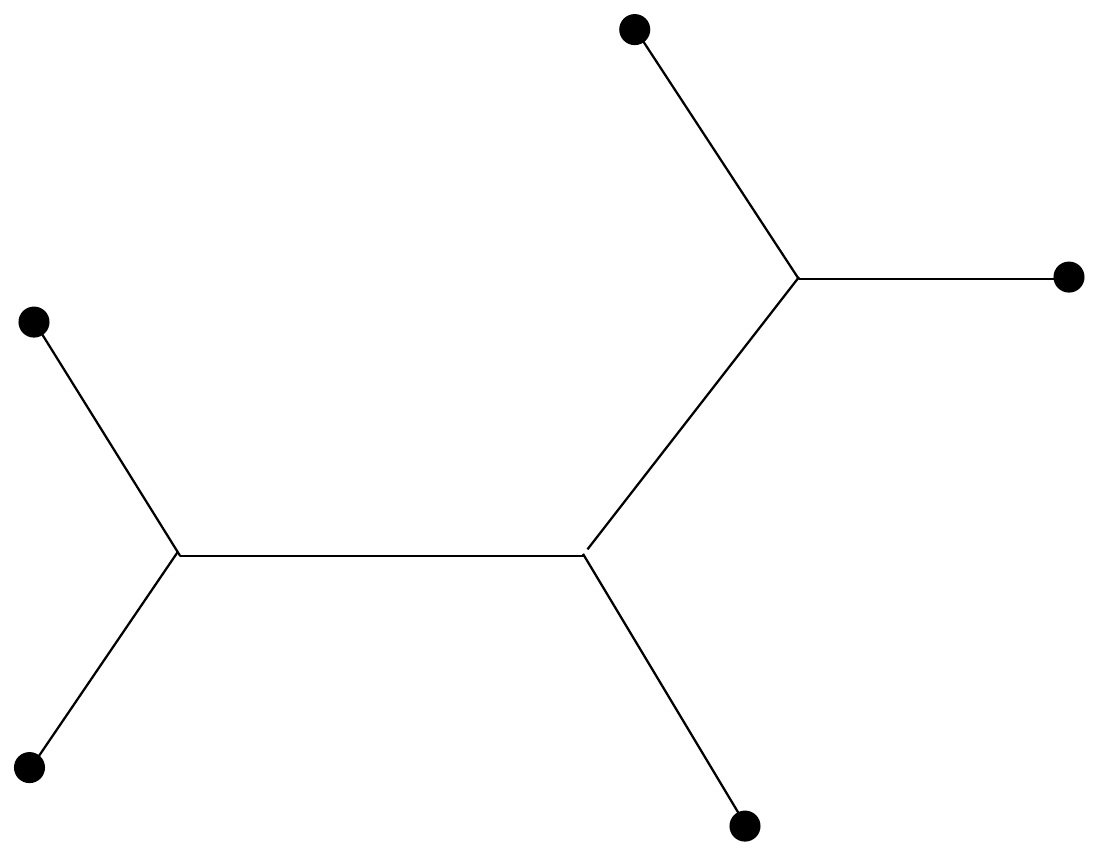
\includegraphics[width=4.64 cm]{figures/fig5_p35_tree_gamma}
\end{center}

复合 $m_k=m_k^{FO(X^\vee,\omega)}$ 由标准公式给出，但此时我们计数的是 a)--d) 所描述的曲面 $S$。权重 $q^{\langle[S],[\omega]\rangle}$ 可以写成
\[
  \exp\Bigl(-\frac{1}{\eps}\sum_\beta \operatorname{var}_{p^\vee(S_\beta)}f_\beta\Bigr),
\]
其中 $f_\beta=f_{i(\beta)}-f_{j(\beta)}$，而 $\operatorname{var}$ 是函数沿梯度流线的（正）变差。

Fukaya--Oh 范畴中对象序列的横截性条件，可以与 Fukaya 范畴的情形类似地表述。

读者可以把我们的讨论与 \cite{FuO} 中的讨论作比较。$p^\vee$ 的纤维是「小」环面（尺度为 $O(\eta)$）。底 $Y$ 是「大」的（尺度为 $O(1)$）。因此，拉格朗日流形接近于 $p^\vee$ 的零截面。这与 \cite{FuO} 中考虑的情形类似。事实上，\cite{FuO} 的作者研究了 $\F(\Tstar_Y)$ 的 $\Ainf$-子范畴（其中 $Y$ 是任意光滑紧流形），其对象 $(L,\rho)$ 满足 $L=\eta\operatorname{graph}(df)$，$f:Y\to\R$ 是光滑函数。换言之，他们考虑的是自然投影 $\Tstar_Y\to Y$ 的、接近于零截面的拉格朗日截面。当 $\eta\to0$ 时，伪全纯圆盘沿 $p^\vee$ 的纤维被「拉伸」，因此看起来就像上面描述的曲面 $S$。于是 Fukaya 范畴的高阶复合「逼近」复合 $m_k^{FO(X^\vee,\omega)}$。\cite{FuO} 在 $X^\vee$ 换成 $\Tstar_Y$ 的情形证明了这一点。\cite{FuO} 的讨论在我们的情形同样适用。

\begin{rmk}
我们可以推广 Fukaya--Oh 范畴，考虑 $X^\vee$ 中不必是 $Y$ 的非分歧覆盖的拉格朗日子流形。例如，可以试着往 $FO(X^\vee)$ 中添加新对象，即投影 $p^\vee:X^\vee\to Y$ 的纤维（拉格朗日环面）上的局部系统。看来借助这些对象可以走得比横截对象远得多。例如，在带奇纤维的环面纤维化的一般情形，可以论证：对几乎所有的 $y\in Y$，不存在以环面 $(p^\vee)^{-1}(y)$ 为边界的极限全纯圆盘。这样的点 $y$ 之集是 $Y$ 中可数个超曲面之并 $Z$ 的补集（这可由 $\dim(Y^{sing})=\dim(Y)-2$ 推出）。于是我们得到一大批真正的对象，且不带寄生的复合 $m_0$。整体图景似乎相当复杂，因为例子表明子集 $Z$ 处处稠密。这大概与某个神秘的非阿贝尔 $1$-余圈有关，我们将在稍后 \S7.1 的注中讨论。
\end{rmk}

\begin{yizhu}[原文的几处排印笔误]
原文中有三处小疵，译文已按数学意义处理：其一，第 30 页定义 $\MM(\dots)$ 时写 $[\phi]=\beta$，按上下文应为 $[\psi]=\beta$（$\psi$ 才是曲面映射）；其二，第 31 页的 Fredholm 指标式中求和指标写作 $i$（$\sum_{0\le i\le m-1}\deg x_{i_p}$），与前后的 $p$ 混用；其三，第 34 页条件 b) 有一处衍字，原文作「$S=(\cup_\alpha T_\alpha)\cup(\cup_\beta S_\beta)$ where and $T_\alpha$ are \dots」。
\end{yizhu}

% [原文 p28–p35（注 15 末句续至 p36 首 5 行）]
